\documentclass{report}
\usepackage{amsmath}
\usepackage{amsthm}
\usepackage{amssymb}
\usepackage[utf8]{inputenc} 
\usepackage{graphicx}
\usepackage{mathtools}
\usepackage{floatrow}
\usepackage{float}

\usepackage{color}
\definecolor{red}{rgb}{1,0,0}

\usepackage{tabularx}

\newtheorem{mydef}{Definition}
\newtheorem{myexample}{Beispiel}
\newtheorem{myproof}{Beweis}
\newtheorem{axiom}{Axiom}
\newtheorem{satz}{Satz}

% sets of numbers
\newcommand{\N}{{\mathbb N}}
\newcommand{\Z}{{\mathbb Z}}
\newcommand{\Q}{{\mathbb Q}}
\newcommand{\R}{{\mathbb R}}
\newcommand{\C}{{\mathbb C}}

\title{Analysis}
\author{Martin Schmidli}

\begin{document}
\maketitle
\chapter{Folgen und Grenzen}
\section{Definition von Folgen}
Betrachten wir Zahlenfolgen wie
\begin{enumerate}
\item $3, 7, 11, 15, 19, \ldots$
\item $16, 8, 4, 2, 1 , \frac{1}{2}, \ldots$
\item $1, -3, 9, -27, 81,\ldots$
\item $1, 1, 2, 3, 5, 8, 13, 21, ...$
\end{enumerate}
So fällt einerseits die Gesetzmässigkeit und andererseits ein immer vorhandenes erstes Element auf.\\
\\
Bezeichnen wir allgemeine Folgen mit
\begin{equation*}a_1 a_2 a_3 a_4 \ldots\end{equation*}
so finden wir bei
\begin{enumerate}
\item
$a_n = 4n -1 (n\in /N)$ das \underline{explizites Gesetz} oder\\
$a_n + 1 = a_n + 4$ und $a_1 = 3$ das \underline{rekursives Gesetz}.
\item
$b_n = 2^{5-n}$ oder \\
$b+1 = \frac{bn}{2}$ und $b_1 = 16$
\item
$c_n = (-3)^{n-1}$\\
Die Folge ist \underline{alternierend}, das heisst + und - wechseln sich ab. 
\item
$d_n = d_{n-1}+ d_{n-2}$ und $d_1 = 1, d_2 = 1$
heisst \underline{Fibonacci-Folge}
\end{enumerate}
\newpage
\begin{mydef}Eine \underline{Folge} ist eine Funktion mit $\N$ als Definitionsmenge\end{mydef}
Anstatt $f(n)$ schreiben wir bei Folgen $a_n$
\begin{myexample}
	\begin{enumerate}
		\item
		$a_n = 3n + 5$\\ 
		Also $8, 11, 14,17, \ldots$
		\item
		$b_n+1 = (-2)b_n$ und $b_1 = -3$ also\\
		$6, -12, 24, -48$
		\item
		$c_n + 1 = c_n + n$ und $c_1 = 4$ also\\
		$c_2 = c_1 + 1 = 5$\\
		$c_3 = c_2 + 2 = 7$\\
		$c_4 = c_3 + 3 = 10$\\
		etc.
	\end{enumerate}
\end{myexample}
\newpage
\section{Teilsummen}
\begin{mydef}
	Bei einer \underline{Arithmetischen Folge (AF)} ist die Differenz zweier aufeinanderfolgender Zahlen immer gleich.
\end{mydef}
\begin{myexample}
	\begin{enumerate}
		\item
			$2, 7 ,12, 17, \ldots \to d = 5$
		\item
			$10, 6 , 2, -2, -6, \ldots \to d = -4$
	\end{enumerate}
\end{myexample}
\noindent
Allgemein ist eine AF
\begin{equation*}a_1,a_1+d,a_1+2d,a_3+3d \ldots,a_1+(n-1)d\end{equation*}
und damit die Teilsumme
\begin{eqnarray*}s_n = a_1 + a_1+d + a_1+2d + a_3+3d \ldots + a_1+(n-1)d\\
\end{eqnarray*}
aber auch 
\begin{equation*}s_n = a_n+a_n -d + a_n + a_n -2d + \ldots + a_n-(n-1)d\end{equation*}
und damit
\begin{eqnarray*}
	2s_n = n(a_1+a_n)\\
	s_n = \frac{n}{2}(a_1+a_n)
\end{eqnarray*}
\begin{myexample}
Wollen wir
\begin{equation*}1 + 2 + 3 + 4 + ... + 100\end{equation*}
berechnen, so greifen wir auf die Idee von Carl Friedrich Gauss (1777 bis 1855, Göttingen) zurück.
\begin{eqnarray}s_{100} & = & (1 + 100) + (2 + 99) + ... + (50 + 51) \nonumber \\
& = & 50 \cdot 101 \nonumber \\
& = & 5050\end{eqnarray}
\end{myexample}
\begin{myexample}
	\begin{eqnarray*}
		530 &=& 4 + 7 + 10 + \ldots + a_{30}\\
		\shortintertext{Es ist}
		a_n &=& 3_n + 1\\
		\shortintertext{also}
		a_30 &=& 91
		\shortintertext{und so}
		s_30 &=& \frac{30}{2}(4+91)\\
		&=& 1435
	\end{eqnarray*}
\end{myexample}
Wollen wir
\begin{equation*}s_n = \frac{1}{2 \cdot 5} + \frac{1}{5 \cdot 8} + \frac{1}{8 \cdot 11} + ... + a_n\end{equation*}
berechnen, so bestimmen wir die \underline{Teilsummenfolge}.
\begin{eqnarray}s_1 & = & \frac{1}{10}\\
s_2 & = & \frac{1}{10} + \frac{1}{5 \cdot 8} = \frac{8 + 2}{2 \cdot 5 \cdot 8} = \frac{10}{80} = \frac{1}{8} \textcolor{red}{ = \frac{2}{16}}\\
s_3 & = & \frac{1}{8} + \frac{1}{8 \cdot 11} = \frac{11 + 1}{8 \cdot 11} = \frac{12}{8 \cdot 11} = \frac{3}{22}\\
s_4 & = & \frac{3}{22} + \frac{1}{11 \cdot 14} = \frac{42 + 2}{2 \cdot 11 \cdot 14} = \frac{2}{14} = \frac{1}{7} \textcolor{red}{ = \frac{4}{28}}\end{eqnarray}
also finden wir
\begin{equation*}s_n = \frac{n}{6n + 4}\end{equation*}
Wir beweisen mit vollständiger Induktion.
\begin{myproof}\begin{enumerate}
\item \label{proof:teilsummenfolge-1} Behauptung ist für $n=1$ wahr, denn
\begin{equation*}s_1 = \frac{1}{10}\end{equation*}
und $s_n$ wird mit $n=1$ zu
\begin{equation*}s_1 = \frac{1}{6 \cdot 1 + 4} = \frac{1}{10}\end{equation*}
\item \label{proof:teilsummenfolge-2} Voraussetzung: 
\begin{equation*}s_n = \frac{n}{6n+4}\end{equation*}
Behauptung:
\begin{equation*}s_{n+1} = \frac{n+1}{6(n+1) + 4} = \frac{n+1}{6n+10}\end{equation*}
Beweis:
\begin{equation*}s_{n+1} = s_n + a_{n+1}\end{equation*}
und wir müssen $a_{n+1}$ bestimmen. Es ist
\begin{equation*}a_n = \frac{1}{(3n-1)(3n+2)}\end{equation*}
, also
\begin{eqnarray}a_{n+1} & = & \frac{1}{(3(n+1)-1)(3(n+1)+2)} \\
& = & \frac{1}{(3n+2)(3n+5)}\end{eqnarray}
Somit ist
\begin{eqnarray}s_{n+1} & = & \frac{n}{6n+4} + \frac{1}{(3n+2)(3n+5)} \\
& = & \frac{n}{2(3n+2)} + \frac{1}{(3n+2)(3n+5)} \\
& = & \frac{3n^2+5n+2}{2(3n+2)(3n+5)} \\
& = & \frac{(3n+2)(n+1)}{2(3n+2)(3n+5)} \\
& = & \frac{n+1}{2(3n+5)} = \frac{n+1}{6n+10}\end{eqnarray}
\item Nach (\ref{proof:teilsummenfolge-1}) ist die Behauptung für $n=1$ wahr und nach (\ref{proof:teilsummenfolge-2}) für $n+1$, also für $n=2$ usw. Also ist die Behauptung für alle $\mathbb{N}$ wahr.
\end{enumerate}\end{myproof}
Natürlich finden wir auch sofort
\begin{equation*}\sum_{k=1}^{n} k = 1 + 2 + ... + n = (1+n)\frac{n}{2}\end{equation*}
Teilsummen schreiben wir mit dem Summenzeichen $\sum$
\begin{myexample}
	\begin{enumerate}
		\item
			\begin{eqnarray*}
				\sum_{n=1}^{100} 4n-1 &=& 3+7+10+\ldots+399\\
				&=& 50(3+399)\\
				&=& 50(402)\\
				&=& 20'100
			\end{eqnarray*}
			Summe $4n-1$, n von 1 = 100
		\item
			\begin{equation*}
				\sum_{k=1}^{10} 2^{3-k} = 4 + 2 + 1 + \ldots + \frac{1}{128}
			\end{equation*}
		\item
			\begin{equation*}
				\sum_{j=1}^{5} ajx^j  = a_1x + a_2x^2 + \ldots + a_5x^5
			\end{equation*}			
	\end{enumerate}
\end{myexample}
\newpage
\section{Grenzwerte}
Betrachten wir die Folge
\begin{equation*}a_n = (-1)^{n+1}(1+\frac{1}{n})\end{equation*}
so erhalten wir
\begin{equation*}
	2, -1.5,1.3\overline{3}, -1.25, 1.2,-1,1\overline{6}, \ldots
\end{equation*}
Zeichnen wir die Werte auf der Zahlengerade
\\\\ BILD TODO\\\\
so sehen wir zwei \underline{Häufungswerte} 1 und -1
\begin{mydef}Wir nennen
\begin{equation*}U_\epsilon(a) := [a-\epsilon; a + \epsilon]; \epsilon > 0\end{equation*}
eine \underline{$\epsilon$-Umgebung} von $a \in \R$.\end{mydef}
\noindent
Wählen wir einen kleinen $\epsilon$ -Wert so sollen unendlich-viele Zahlen in $U_\epsilon(a)$ liegen.
\begin{mydef}
	Eine Zahl a heisst \underline{Häufungswert} einer Folge $a_n$ wenn für jedes $\epsilon > 0$ unendlich-viele Folgenglieder in $U_{\epsilon}(a)$ liegen.
\end{mydef}
\begin{myexample}
\begin{enumerate}
	\item
	\begin{eqnarray}
	a_n &=& 2n + 1\\
	& \rightarrow& 3,5,7,9,\ldots\\
	\end{eqnarray}
	also kein Häufungswert
	\item 
	\begin{eqnarray}
	a_n & = & \frac{n+1}{n} \nonumber \\
	& \rightarrow & 2, 1.5, 1.\bar{3}, 1.25, 1.2, 1.16, 1.\bar{142857}\end{eqnarray}
	also ist 1 ein Häufungswert.
	\item \begin{eqnarray}b_n & = & 4n + 1 \nonumber \\
	& \rightarrow & 5, 9, 13, 17, ...\end{eqnarray}
	Also kein Häufungswert.
\end{enumerate}
\end{myexample}
\noindent
Besitzt eine Folge genau einen einzigen Häufungswert, so nennen wir diesen den \underline{Limes} (Grenzwert) der Folge und schreiben
\begin{equation*}\boxed{\lim_{n \to \infty}a_n = a }\end{equation*}
\begin{myexample}
\begin{enumerate}
\item
	\begin{eqnarray*}
		a_n &=& (-1)^n\frac{1}{n}\\
		&\rightarrow& -1, \frac{1}{2}, -\frac{1}{3}, \frac{1}{4}, -\frac{1}{5}, \ldots\\
		\lim_{n \to \infty}(-1)^n\frac{1}{n} &=& 0 
	\end{eqnarray*}
\item
	\begin{eqnarray*}
		b_n &=& (2)^{3-n}\\
		&\rightarrow& 4,2,1,\frac{1}{2},\frac{1}{4}, \ldots\\
		\lim_{n \to \infty}(2)^{3-n} &=& 0 
	\end{eqnarray*}
\item
	\begin{eqnarray*}
		c_n &=& 3+\frac{1}{n^2}\\
		&\rightarrow& 4,3+\frac{1}{4},3+\frac{1}{9},3+\frac{1}{16}, \ldots\\
		\lim_{n \to \infty}3+\frac{1}{n^2} &=& 3\\ 
	\end{eqnarray*} 
\item
	\begin{equation*}\lim_{n \to \infty}\frac{n+1}{n}=1\end{equation*}
\item 
	\begin{equation*}\lim_{n \to \infty}(-1)^n(2+\frac{1}{n})\end{equation*}
\item 
	\begin{equation*}\lim_{n \to \infty}\frac{1}{n}=0\end{equation*}
\end{enumerate}
\end{myexample}
\begin{mydef}\underline{Definition von Couchy}\\Im Folgenden die Definition des Limes nach Cauchy (Louis Augustin Cauchy, 1789 bis 1857, Paris, Schweiz, Prag):\\
Eine Zahlenfolge $(a_n)$ besitzt den Grenzwert $a$, wenn für alle $\epsilon > 0$ von einem bestimmten $n$ an, alle weiteren Folgenglieder in $U_\epsilon(a)$ liegen:
\begin{equation*}\epsilon \in \mathbb{R}, n_0 \in \mathbb{N}: \forall \epsilon > 0\exists n_0 \forall n (n > n_0 \to |a_n-a| < \epsilon)\end{equation*}\end{mydef}
\begin{myexample}$a_n = \frac{5}{n}$ hat Grenzwert $a=0$\\
Ist $\epsilon = \frac{1}{100}$, so wird $n_0 = 500$, denn von $a_{501}$ an sind alle Folgenglieder zwischen $0,01$ und $0$.\end{myexample}
\begin{mydef}Besitzt eine Folge $a_n$ einen Grenzwert, so heisst sie \underline{konvergent}, andernfalls \underline{divergent}. Folgen mit Grenzwert $0$ heissen \underline{Nullfolgen}.\end{mydef}
\begin{myexample}Nullfolgen\\
	\begin{tabularx}{\textwidth}{XX}
		\begin{equation*}a_n = \frac{1}{n}\end{equation*}&\begin{equation*}b_n = \frac{1}{n^2}\end{equation*}\\
		\begin{equation*}c_n = \frac{1}{n^3}\end{equation*}&\begin{equation*}d_n = \frac{2}{n}\end{equation*}\\
		\begin{equation*}e_n = \frac{3}{n^2}\end{equation*}&\begin{equation*}f_n = \frac{4}{n^3}\end{equation*}
	\end{tabularx}
\end{myexample}
\noindent
Suchen wir
\begin{eqnarray*} 
	\lim_{n \to \infty} \frac{4n+1}{n}\\	
	\shortintertext{so formen wir um}\\
	\frac{4n}{n}+ \frac{1}{n} = 4 + \frac{1}{n}\\
	\shortintertext{also}\\
	\lim_{n \to \infty} \frac{4n +1}{n} = \lim_{n \to \infty}4+\frac{1}{n} = 4
\end{eqnarray*}
Bei
\begin{eqnarray*}
	\lim_{n \to \infty}\frac{5n+3}{6n-2}\\
	\shortintertext{kürzen wir mit n und erhalten}\\
	\lim_{n \to \infty}\frac{\frac{5n+3}{n}}{\frac{6n-2}{n}} = \lim_{n \to \infty}\frac{5+\frac{3}{n}}{6 -\frac{2}{n}} = \frac{5}{6}
\end{eqnarray*}
\newpage
\begin{myexample}Wir kürzen jeweils mit der Variabel ($n$) mit der höchsten Potenz
\begin{enumerate}
	\item 
	\begin{eqnarray*}
		&&\lim_{n \to \infty} \frac{2n^2-3n+1}{3n^2+5n-7} \\
		&=& \lim_{n \to \infty}\frac{\frac{2n^2}{n^2}-\frac{3n}{n^2}+\frac{1}{n^2}}{\frac{3n^2}{n^2}+\frac{5n}{n^2}-\frac{7}{n^2}} \\
		&=& \lim_{n \to \infty}\frac{2-\frac{3}{n}+\frac{1}{n^2}}{3+\frac{5}{n}-\frac{7}{n^2}} = \frac{2}{3}
	\end{eqnarray*}
	\item
	\begin{eqnarray*}
		&&\lim_{n \to \infty} \frac{2n^3+4}{n^2-5}\\
		&=&\lim_{n \to \infty} \frac{\frac{2n^3}{n^3}+ \frac{4}{n^3}}{\frac{n^2}{n^3}-\frac{5}{n^3}}\\
		&=&\lim_{n \to \infty} \frac{2+ \frac{4}{n^3}}{\frac{1}{n}-\frac{5}{n^3}}\\
	\end{eqnarray*}
	$\frac{2}{0}$ ist nicht erlaubt\\
	Ist divergent, es existiert kein Grenzwert. 
	\item \begin{eqnarray*}
	&&\lim_{n \to \infty}\frac{\sqrt{n}+\sqrt{n-1}}{\sqrt{n}-\sqrt{2n-1}} \\
	& = & \lim_{n \to \infty}\frac{\frac{\sqrt{n}}{\sqrt{n}}+\frac{\sqrt{n-1}}{\sqrt{n}}}{\frac{\sqrt{n}}{\sqrt{n}}-\frac{\sqrt{2n-1}}{\sqrt{n}}} \\
	&=& \lim_{n \to \infty}\frac{1+\frac{\sqrt{n-1}}{\sqrt{n}}}{1-\frac{\sqrt{2n-1}}{\sqrt{n}}} \nonumber \\
	&=& \lim_{n \to \infty}\frac{1+\sqrt{1-\frac{1}{n}}}{1-\sqrt{2-\frac{1}{n}}} \\
	&=& \frac{1+\sqrt{1}}{1-\sqrt{2}} \\
	&=& \frac{2}{1-\sqrt{2}}
	\end{eqnarray*}
\end{enumerate}\end{myexample}
\newpage
\noindent
Um
\begin{equation*}\lim_{n \to \infty} (1+\frac{1}{n})^n\end{equation*}
zu berechnen, bestimmen wir
\begin{equation*}a_{100} = 2,70481 \ldots, a_{1000} = 2,7169\ldots\end{equation*}
und finden, dass die Folge beschränkt ist. Es ist
\begin{equation*}\boxed{\lim_{n \to \infty} (1 + \frac{1}{n})^n = e}\end{equation*}
und $e = 2,71828...$ ist irrational und transzendent.
\begin{myexample}
\begin{enumerate}
\item \begin{equation*}\lim_{n \to \infty} ( 1 + \frac{1}{5n})^{5n} = e\end{equation*}
\item \begin{equation*}\lim_{n \to \infty} ( 1 + \frac{1}{\frac{n}{3}})^{\frac{n}{3}} = e\end{equation*}
\item 
	\begin{eqnarray*}
		&&\lim_{n \to \infty} ( 1 + \frac{1}{n})^{4n} \\
		&=& \lim_{n \to \infty}[ ( 1 + \frac{1}{n})^{n}]^4\\ 
		&=& e^4
	\end{eqnarray*}
\item
\begin{equation*}\lim_{n \to \infty} ( 1 + \frac{k}{n})^n, k \in \mathbb{Z}\end{equation*}
Wir überlegen, dass
\begin{equation*}1 + \frac{k}{n}  =1 + \frac{1}{\frac{n}{k}}\end{equation*}
und finden
\begin{equation*}\lim_{n \to \infty} ( 1 + \frac{1}{\frac{n}{k}})^\frac{n}{k} = e\end{equation*}
Weiter ist dann
\begin{equation*}\lim_{n \to \infty} (1 + \frac{k}{n})^n = \lim_{n \to \infty}[(1 + \frac{k}{\frac{n}{k}})^\frac{n}{k}]^k = e^k\end{equation*}
ist $k = -1$, so
\begin{equation*}\lim_{n \to \infty} (1 - \frac{1}{n})^n = \lim_{n \to \infty} (1 + \frac{-1}{n})^n = e^{-1} = \frac{1}{e}\end{equation*}
Zusammengefasst
\begin{eqnarray}\lim_{n \to \infty} (1 + \frac{1}{n})^n & = & e\\
\lim_{n \to \infty} (1 - \frac{1}{n})^n & = & \frac{1}{e} = e^{-1}\\
\lim_{n \to \infty} (1 + \frac{k}{n})^n & = & e^k, k \in \mathbb{Z}\end{eqnarray}
\end{enumerate}\end{myexample}
\newpage

\chapter{Differentialrechnung}
\section{Tangentenproblem}
Wir betrachten eine stetige Funktion
\begin{equation*}f: D_f \mapsto \mathbb{R}\end{equation*}
und suchen die Steigung der Tangente an dem Graphen an der Stelle $x_0 \in D_f$.
\\\\TODO\\\\
Die Tangente ist eine spezielle Lage der Sekante. Die Steigung der Sekante ist
\begin{equation*}m_s = \frac{\Delta y}{\Delta x} = \frac{f(x_0 + h) - f(x_0)}{h}\end{equation*}
, was wir den \underline{Differenzenquotient} nennen. Wird $h$ immer kleiner, so nähert sich die Sekante der Tangente. Also ist die Tangentensteigung
\begin{equation*}m_t = \lim_{h \to 0} \frac{f(x_0 + h) - f(x_0)}{h}\end{equation*}
\begin{mydef}Wir nennen
\begin{equation*}\frac{\mathrm{d}y}{\mathrm{d}x} := \lim_{h \to 0} \frac{f(x_0 + h) - f(x_0)}{h} \quad \mbox{("dy nach dx")}\end{equation*}
den \underline{Differentialquotienten}.\end{mydef}
\begin{myexample}
	\begin{enumerate}
	\item
	Welche Gleichung hat die Tangte in $x_0 = 2$ an den Graphen von $f(x) = x^3$ mit $Df = \R$?
	Mit
	\begin{eqnarray*}
		f(x_0) &=& 2^3 = 8
		\shortintertext{und}
		f(x_0+h) &=& (2+h)^3
		\shortintertext{Mithilfe des Pascalschen Dreiecks finden wir}
		&=& 2^3 + 3\cdot 2^2h + 3 \cdot 2h^2 + h^3\\
		&=& 8 + 12h + 6h^2 + h^3
		\shortintertext{damit wird}
		\frac{dy}{dx} &=& \lim_{h\to 0} \frac{8 + 12h + 6h^2 + h^3-8}{h}\\
		&=& \lim_{h \to 0} \frac{12h+6h^2 + h^3}{h}\\
		&=& \lim_{h \to 0} 12 + 6h + h^2\\
		&=& 12
	\end{eqnarray*}
	\item
	$g(x) = \frac{1}{x}$ mit $D_g = \R \\ {0}$ und $x_0 = 3$\\
	Mit
	\begin{eqnarray*}
		g(x_0)&=& \frac{1}{3}
		\shortintertext{und}
		g(x_0+h) &=& \frac{1}{3+h}
		\shortintertext{wird}
		\frac{dy}{dx}  &=& \lim_{h \to 0} frac{\frac{1}{3+h}-\frac{1}{3}}{h}\\
		&=& \lim_{h \to 0} \frac{\frac{3-(3+h)}{3(3+h)}}{h}\\
		&=& \lim_{h \to 0} \frac{-h}{3(3+h)} \cdot \frac{1}{h}\\
		&=& \lim_{h \to 0} \frac{-1}{3(3+h)}\\
		&=& -\frac{1}{9}
	\end{eqnarray*}
	\end{enumerate}
\end{myexample}
\newpage
\noindent
Welche Gleichung hat die Tangente in $x_0 = 4$ an den Graphen von $f(x) = x^2$ mit $Df = \R$?
\begin{eqnarray*}
	\frac{dy}{dx} &=& \lim_{h \to 0} \frac{(4+h)^2-4^2}{h}\\
	&=& \lim_{h \to 0} \frac{8h + h^2}{h}\\
	&=& \lim_{h \to 0} 8+h\\
	m&=&8
\end{eqnarray*}
Der Punkt $P(4/16)$ liegt auf t.\\
In $y = mxy + q$\\
erhalten wir
\begin{eqnarray*}
	16 = 8 \cdot 4 + q\\
	q = -16
	\shortintertext{und so}
	t: y = 8x -16
	\shortintertext{Kennen wir $P(x_p/y_p)$ einer Geraden $g: y= mx + q$ so ist}
	y_p = mx_p + q\\
	y_p -mx_p = q\\
	\shortintertext{also}
	q: y = mx + y_p -mx_p\\
	y -y_p = mx - mx_p\\
	\boxed{y-y_p = m(x-x_p)}
	\shortintertext{Wir nennen diese Form Punkt Steigungsform}
\end{eqnarray*}
\newpage
\section{Ableitung}
Wir berechnen $\frac{dy}{dx}$ allgemein für ein beliebiges $x_0$\\
Ist 
\begin{eqnarray}
&&f:\mathbb{R} \mapsto \mathbb{R}_0^+ \text{ mit } f(x) = x^2
\shortintertext{so wird} 
 \frac{\mathrm{d}y}{\mathrm{d}x} & = & \lim_{h \to 0} \frac{(x_0)^2 - x_0^2}{h} \nonumber \\
 & = & \lim_{h \to 0} \frac{x_0^2 + 2x_0h + h^2 -x_0^2}{h}  \nonumber \\
 & = & \lim_{h \to 0} \frac{2x_0h + h^2}{h}  \nonumber \\
 & = & \lim_{h \to 0} 2x_0 + h \nonumber \\
 & = & \underline{2x_0} \end{eqnarray}

Ist $ g:\mathbb{R} \mapsto \mathbb{R}$ mit $ g(x) = x^3$ so wird \begin{eqnarray}
\frac{\mathrm{d}y}{\mathrm{d}x} & = & \lim_{h \to 0} \frac{(x_0)^3 - x_0^3}{h} \nonumber \\
& = & \lim_{h \to 0} \frac{1x_0^3 + 3x_0^2h + 3 x_0h^2 + h^3 + x_0^3}{h} \nonumber \\
& = & \lim_{h \to 0} 3x_0^2 + 3x_0h + h^2  \nonumber \\
& = & \underline{3x_0^2} \end{eqnarray}
Ist $ h:\mathbb{R} \mapsto \{2\}$ mit $ h(x) = 2$, %graph29 1
So ist $ \frac{\mathrm{d}y}{\mathrm{d}x} = 0$
Ist $ i:\mathbb{R} \mapsto \mathbb{R}$ mit $ i(x) = x$ %graph29 2
so ist $\frac{\mathrm{d}y}{\mathrm{d}x} = 1$\\
Wie haben also jedem $x_0 \in D_f$ den Differentialquotienten zugeordnet und so eine Funktion gebildet. Schreiben wir $x$ anstatt $x_0$, so erhalten wir die \underline{1. Ableitung}.
\begin{mydef} Ist $f$ eine differenzierbare Funktion, so heisst \begin{equation*}f'(x) = \lim_{h \to 0} \frac{f(x+h) -f(x)}{h}\end{equation*}
die \underline{1. Ableitung} von f.\end{mydef}
Wir kennen also schon
\begin{eqnarray}
f(x) = k & \to & f'(x) = 0 \quad  (k \in \mathbb{R}) \\
f(x) = x & \to & f'(x) = 1 \\
f(x) = x^2 & \to & f'(x) = 2x \\
f(x) = x^3 & \to & f'(x) = 3x^2 \end{eqnarray}
\begin{satz}
Ist
\begin{equation*}f(x) = x^n \mapsto f'(x) = n \cdot x^{n-1}, n \in \mathbb{N}\end{equation*}\end{satz}
\begin{myproof}Mit \begin{eqnarray}f(x+h) & = & (x+h)^n \nonumber \\
& = & x^n + nx^{n-1}h + \frac{n(n-1)}{2}x^{n-2}h^2+ ... + nxh^{n-1} + h^n\end{eqnarray}
wird
\begin{eqnarray}f(x+h)-f(x) & = & nx^{n-1}h + \frac{n(n-1)}{2}x^{n-2}h^2+ ... + h^n \nonumber \\
& = & h(nx^{n-1}+\frac{n(n-1)}{2}x^{n-2}h + ... + h^{n-1})\end{eqnarray}
und so
\begin{eqnarray}f'(x) & = & \lim_{h \to 0}(nx^{n-1} + \frac{n(n-1)}{2}x^{n-2}h + ... + h^{n-1}) \nonumber \\
& = & nx^{n-1}\end{eqnarray} \qed
\end{myproof}
\begin{myexample}
\begin{equation*}f(x) = x^5-x^3 \to f'(x) = 5x^4-3x^2\end{equation*}
\end{myexample}
\newpage
\subsubsection{Eigenschaften der Ableitung}
Die Ableitung ist ein Grenzwert und deshalb können wir die Grenzwertsätze zum teil übertragen:
\begin{equation*}k \in \mathbb{R}: (k \cdot f(x))' = k \cdot f'(x)\end{equation*}
\begin{equation*}(f(x) + g(x))' = f'(x) + g'(x)\end{equation*}
\begin{myexample}Wir wenden diese Sätze an Beispielen an:
\begin{enumerate}
\item
\begin{eqnarray*}
	f(x)&=& x^6 + x^4 + x^2 + 5\\
	\to f'(x) &=&  (x^6)'+(x^4)'+(x^2)'+(5)'\\
	 &=& 6x^5 + 4x^3 + 2x 
\end{eqnarray*}
\item
\begin{eqnarray*}
	g(x) &=& 4x^3 + 2x^2 + 6x\\
	\to g'(x) &=& 4(x^3)' + 2(x^2)' + 6(x)'\\
	&=& 4 \cdot 3x^2 + 2 \cdot 2x +6 \cdot 1\\
	&=& 12x^2 + 4x + 6
\end{eqnarray*}
\item 
\begin{eqnarray*}
f(x) & = & 5x^4 + 2x^3 - 6x + 8 \nonumber \\
\to f'(x) & = & (5x^4)' + (2x^3)' - (6x)' + (8)' \nonumber \\
& = & 5(x^4)' + 2(x^3)' - 6(x)' + 0 \nonumber \\
& = & 5(4x^3) + 2(3x^2) - 6 \nonumber \\
& = & 20x^3 + 6x^2 - 6
\end{eqnarray*}
\item \begin{eqnarray}g(x) & = & \frac{x^3}{7} + \frac{x^2}{9} - \frac{x}{2} \nonumber \\
& = & \frac{1}{7}x^3 + \frac{1}{9}x^2 - \frac{1}{2}x \nonumber \\
\to g'(x) & = & \frac{3x^2}{7} + \frac{2x}{9} - \frac{1}{2}\end{eqnarray}
\item
\begin{eqnarray*}
	h(x) &=& (x^2+2)(x-1)\\
	&=& x^3 -x^2 + 2x -2\\
	\to h'(x) &=& 3x^2 -2x + 2
\end{eqnarray*}
\end{enumerate}
\end{myexample}
\noindent
Treten in der Funktion noch Parameter auf, so wird oft die Schreibweise nach Leibniz gewählt.
\begin{myexample}
	\begin{eqnarray*}
		v &=& at^2 + a^2t + a^3t^3\\
		\to \frac{dv}{dt} &=& a \cdot 2t + a^2 + a^3 \cdot 3t^2\\
		&=& 2at + a^2 + 3a^3t^2
	\end{eqnarray*}
\end{myexample}
\newpage
\section{Horizontale Tangenten}
Der Graph einer Funktion $f$ kann Punkte mit horizontaler Tangente besitzen.
\begin{equation*}f'(x)=0\end{equation*}
Bild Todo\\
\begin{itemize}
\item $H_1, H_2$ sind \underline{Hochpunkten} 
\item $S$ ist ein \underline{Terrassenpunkt (Scheitelpunkt)} und
\item $T$ ist ein \underline{Tiefpunkt} 
\end{itemize}
Man beachte
\begin{equation*}\text{ein Graph} \not = \text{Funktion}\end{equation*}
Bei einem Graph spricht man von einem ein Hoch (Hochpunkt), bei einer Funktion von einem Maximum.\\
\\
Ist in $x_1$ die Tangente Horizontal, so ist $f'(x_1) = 0$; also können wir mit Hilfe von $f'$ die besonderen Punkte der Graphen finden.
\begin{myexample}
	\begin{enumerate}
		\item
		\begin{eqnarray*}
			f: \R \to \R
			\shortintertext{mit}
			f(x) = x^3 -3x
			\shortintertext{Es ist}
			f'(x) = 3x^2 -3
			\shortintertext{und}
			f'(x) = 0
			\shortintertext{wenn}
			3x^2 -3 = 0\\
			x^2 = 1\\
			x_{1,2} = \pm 1
			\shortintertext{Damit}
			y_1 = f(1) = -2, y_2 = f(-1) = 2
		\end{eqnarray*}
		BILD TODO\\
		Wir suchen einen 3. Punkt\\
		Mit
		\begin{eqnarray*}
			f(0) = 0
			\shortintertext{und}
			x^3 -3x = 0\\
			x(x^2-3) = 0\\
			x_3 = 0, x_4 = \sqrt{3}, x_5 = -\sqrt{3}
		\end{eqnarray*}
		also hat der Graph die Form
		\begin{figure}[ht]
			\centering
			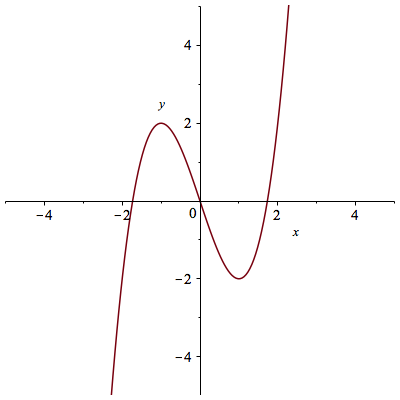
\includegraphics[width=0.7\textwidth]{images/x^3-3x.png}
		\end{figure}
		\item
		\begin{eqnarray*}
			g(x) = x^4 -2x^2
			\shortintertext{bestimme auch die Wertemenge}
			\shortintertext{Es ist}
			g'(x) = 4x^3 -4x
			\shortintertext{und}
			g'(x) = 0
			\shortintertext{wenn}
			4x^3 -4x = 0\\
			4x(x^2 -1) = 0\\
			x_1 = 0, x_2 = 1, x_3 = -1 
			\shortintertext{Wir finden weiter}
			y_1 = g(0) = 0, y_2 = g(1) = -1, y_3 = g(-1) = -1
			\shortintertext{Wir haben die Punkte mit Horizontaler Tangente gefunden  und können diese nun in den Graphen einzeichnen}
		\end{eqnarray*}
		\begin{figure}[ht]
			\centering
			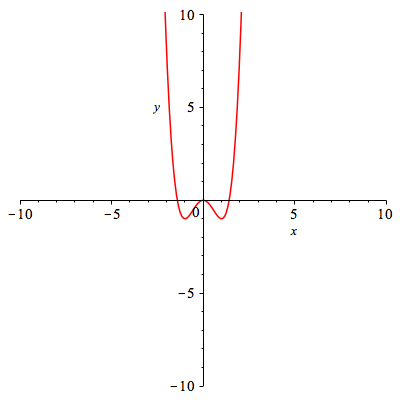
\includegraphics[width=0.7\textwidth]{images/x^4-2x^2.png}
		\end{figure}
		Um den Graphen korrekt zeichnen zu können, suchen wir weitere Punkte.\\
		Wir suchen die Nullstellen
		\begin{eqnarray*}
			x^4 -2x^2 = 0\\
			x^2(x^2-2) = 0\\
			x_1 = 0, x_4 = \sqrt{2}, x_5 = -\sqrt{2}\\
			\text{Wertemenge: Wg} = [-1, \infty[
		\end{eqnarray*}
		% 20.10.2014%
		\newpage
		\item
		\begin{eqnarray*}
			h: \R \ {0} \to R \text{ mit } h(x) = x + \frac{1}{x^2}\\
			\shortintertext{Mit} h(x9 = x+ x^{-2}\\
			\shortintertext{wird}
			h'(x) = 1-2x^{-3} = 1 -\frac{2}{x^3}\\
			\shortintertext{und}
			h'(x) = 0
			\shortintertext{wenn}
			1 = \frac{2}{x^3}\\
			x^3 = \frac{1}{2}\\
			x_1 = \sqrt[3]{\frac{1}{2}} = 1.26\\
			\to y_1 - f(x_1) = 1.9
		\end{eqnarray*}
		\begin{figure}[ht]
			\centering
			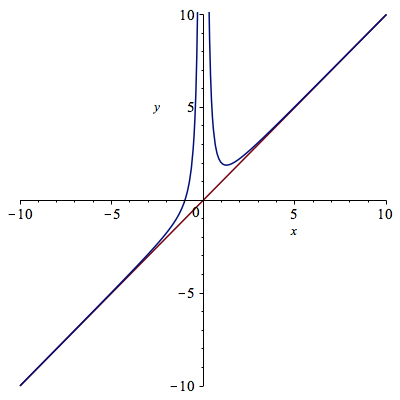
\includegraphics[width=0.7\textwidth]{images/x+x^(-2).png}
		\end{figure}
		Für Grösse $x$ ist $x+ \frac{1}{x^2} \approx x$, also ist $y = x$ die Asymptote.
		\begin{mydef}
			Eine \underline{Asymptote} ist eine Gerade, welcher sich der Graph einer Funktion für sehr grosse $x$ (bzw. sehr kleine $x$) immer mehr nähert.\\
		\end{mydef}
		\underline{Nullstellen:}
		\begin{eqnarray*}
			x + \frac{1}{x^2} &=& 0\\
			x^3 + 1 &=& 0\\
			x^3 &=& -1\\
			x_0 &=& -1
		\end{eqnarray*}
		\newpage
		\item
		\begin{eqnarray*}
			i: \R_0^+ \to \R \text{ mit } i(x) &=& x - \sqrt{x}\\
			\shortintertext{Mit}
			i(x) &=& x - x^{\frac{1}{2}}
			\shortintertext{wird}
			i'(x) &=& 1 - \frac{1}{2}x^{-\frac{1}{2}} = 1 - \frac{1}{2\sqrt{x}}\\
			\shortintertext{und}
			i(x) &=& 0
			\shortintertext{, wenn}
			1 &=& \frac{1}{2\sqrt{x}}\\
			2\sqrt{x} &=& 1\\
			\sqrt{x} &=& \frac{1}{2}\\
			x_1 &=& \frac{1}{4}
			\to y_1 = f(x_1) = -\frac{1}{4}
		\end{eqnarray*}
		\begin{figure}[ht]
			\centering
			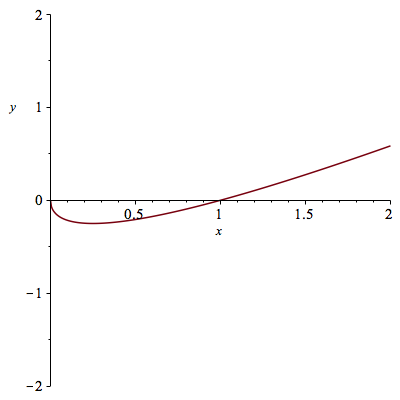
\includegraphics[width=0.7\textwidth]{images/x-sqrt(x).png}
		\end{figure}
		\underline{Nullstellen:}
		\begin{eqnarray*}
			x -x^{\frac{1}{2}} &=& 0\\
			x &=& \sqrt{x}\\
			x^2 &=& x\\
			x^2-x &=& 0\\
			x(x-1) &=& 0\\
			x_2 = 0, x_3 = 1
		\end{eqnarray*}
	\end{enumerate}
\end{myexample}
\newpage
\section{Nullstellen}
Suchen wir die Nullstellen von
\begin{eqnarray*}
	f(x) &=& x^2 -x-30 \text{ mit } Df = \R\\
	\shortintertext{so ist}
	x^2 -x-30 &=& 0\\
	(x+5)(x-6) &=& 0
	\shortintertext{also}
	x_1 = -5, x_2 = 6
\end{eqnarray*}
Bei
\begin{eqnarray*}
	g(x) = x^2-6x+9, Dg = \R
	\shortintertext{wird also}
	x^2 -6x+9 = 0\\
	(x-3)^2 = 0\\
	(x-3)(x-3) = 0\\
	\shortintertext{und so}
	x_1 = 3, x_2 = 3
	\shortintertext{und wir nennen}
	x_{1,2} = 3
\end{eqnarray*}
eine doppelte Nullstelle\\
\\
\underline{Graphen von f und g}\\
\begin{tabularx}{\textwidth}{XX}
	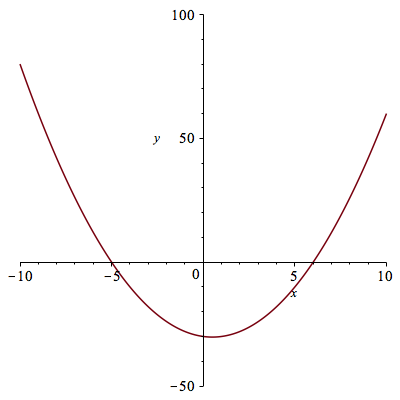
\includegraphics[width=0.5\textwidth]{images/x^2-x-30.png} &
	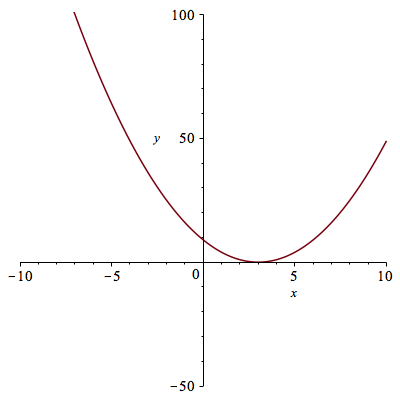
\includegraphics[width=0.5\textwidth]{images/x^2-6x+9.png}
\end{tabularx}
Gg besitzt einen \underline{Berührungspunkt} auf der x-Achse und damit eine horizontale Tangente.\\
\newpage
\noindent
Ist
\begin{equation*}f(x) = (x-2)(x+3)^2 \text{ mit } Df = \R\end{equation*}
So wissen wir sofort, die Nullstelle
\begin{eqnarray*}
	x_1 = 2
	\shortintertext{doppelte Nullstelle}
	x_2 = -3
\end{eqnarray*}
Also berührt Gf bei $x= -3$ die x-Achse.\\
\begin{figure}[ht]
	\centering
	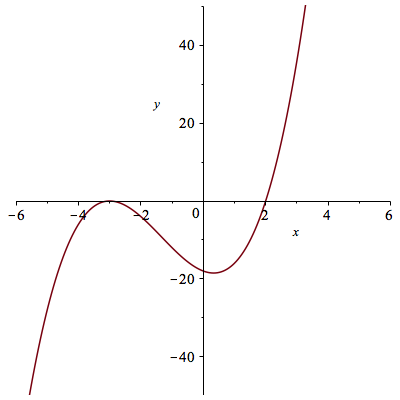
\includegraphics[width=0.7\textwidth]{images/(x-2)(x+3)^2.png}
\end{figure}
Wir wissen
\begin{eqnarray*}f(0) < 0
	\shortintertext{da}
	f(0) &=& (0-2)(0+3)^2\\
	&=& (-2)9\\
	&=& -18
\end{eqnarray*}
\newpage
\noindent
Die Funktion
\begin{equation*}
	g(x) = (x-2)^3 \text{ mit } Dg = \R 
\end{equation*}
besitzt die \underline{dreifache Nullstelle} $x_{1,2,3} = 2$\\
\begin{figure}[ht]
	\centering
	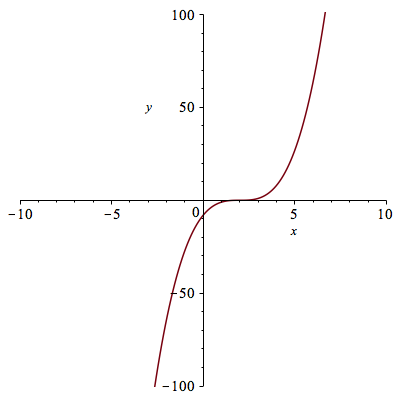
\includegraphics[width=0.7\textwidth]{images/(x-2)^3.png}
\end{figure}
Der Graph besitzt einen Terassenpunkt auf der x-Achse.\\
\newpage
\noindent
Die Funktion
\begin{equation*}h(x) = (x-5)^4 \text{ mit } Dh = \R\end{equation*}
besitzt die vierfache Nullstelle $x_{1,2,3,4} = 5$ und der Graph besitzt bei $x=5$ einen underline{Flachpunkt} auf der x-Achse.\\
\begin{figure}[ht]
	\centering
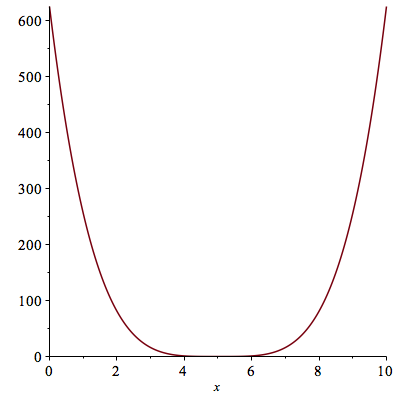
\includegraphics[width=0.7\textwidth]{images/(x-5)^4.png}
\end{figure}
\newpage
\begin{myexample} 
	Skizziere den Graphen von
	\begin{equation*}
		f(x) = (x+4)^2 (x+1)(x-3)^3 \text{ mit } Df = \R 
	\end{equation*}
	Also doppelte Nullstelle bei $x_{1,2} = -4 \to$ Berührungspunkt\\
	einfache Nullstelle bei $x_3 = -1 \to$ Schnittpunkt\\
	dreifache Nullstelle bei $x_{4,5,6} = 3 \to$ Terassenpunkt\\
	\begin{figure}[H]
		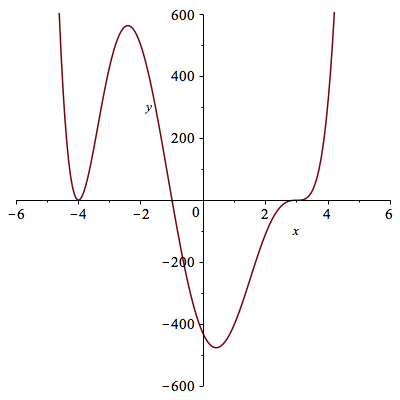
\includegraphics[width=0.7\textwidth]{images/(x+4)^2(x+1)(x-3)^3.png}
	\end{figure}
	unf $f(0) < 0$
\end{myexample}
%26.10.2014%
\newpage
\section{Höhere Ableitung und Kurvendiskussion}
Wenn wir die Ableitung $f'$ einer Funktion erneut ableiten, so erhalten wir die \underline{zweite Ableitung $f''$}. Fahren wir so fort, so erhalten wir $f''',f^(4),f^(5)\ldots$ und schliesslich die \underline{n. Abteilung $f^(n)$}.
\begin{myexample}
	\begin{equation*}
		f: \mathbb{R} \mapsto \mathbb{R} \quad \mbox{mit} \quad f(x) = 4x^3+2x^2 -6x+10
	\end{equation*}
	\begin{eqnarray}
		\to f'(x) & = & 12x^2 + 4x -6 \nonumber \\
		f''(x) & = & 24x + 4 \nonumber \\
		f'''(x) & = & 24 \nonumber \\
		f^{(4)}(x) & = & f^{(5)}(x) = f^{(n)}(x) = 0 
	\end{eqnarray}
\end{myexample}
\begin{mydef}
	Eine Funktion $f: \R \to \R mit$
	\begin{eqnarray*}
		f(x) &=& a_nx^n+a_{n-1}x^{n-1}+\ldots + a_2x^2 + a_1x^1+a_0\\
		f(x) &=& \sum_{k=0}^n a_kx^k
	\end{eqnarray*}
	mit $a_k\in \Q (k=0,1,\ldots,n)$ und $n \in \N$ heisst \underline{ganzrationale Funktion (Polynomfunktion)} mit Grad n.
\end{mydef}
\noindent
Bei ganzrationalen Funktionen n. Grades wird 
\begin{equation*} f^{n+1}(x) = 0\end{equation*}
Welche Informationen für $f'$ erhaten wir von $f''$\\
% BILD TODO
BILD TODO\\
Besitzt der Graph Gf 
\begin{itemize}
\item einen Terassenpunkt $x_2$ so ist $f'(x_2) = 0 \land f''(x_2) = 0$\\
\item einen Hochpunkt $x_3$ so ist $f'(x_3) = 0 \land f''(x_3) < 0$\\
\item einen Tiefpunkt $x_4$, so ist $f'(x_4) = 0 \land f''(x_4) > 0$  
\end{itemize}
f'' gibt Information über die \underline{Krümmung} des Graphen.\\
\begin{tabularx}{\textwidth}{XXX}
	%BILD TODO
	rechts gekrümmt (Konkav) f''(x)<0\\BILD TODO & links gekrümmt (konvex) f''(x)>0 \\BILD TODO & Wendepunkt \\ f''(x) = 0
\end{tabularx}
\subsection{Kurvendiskussion}
Bei einer \underline{Kurvendisskussion} bestimmen wir 
\begin{itemize}
	\item Nullstellen: $f(x) = 0$
	\item Punkte mit horizontalen Tangenten/ Extremalwerte: f'(x) = 0
	\item Wendepunkte: f''(x) = 0 
\end{itemize}
und skizzieren dann den Graphen Gf.
\begin{myexample}
	Diskutiere $f: \R \to \R$ mit $f(x) = x^4 -6x^2 + 8$ und bestimme die Wertemenge.\\
	\\
	\underline{Nullstellen:}
	\begin{eqnarray*}
		x^4 -6x^2 + 8 &=& 0\\
		(x^2 -2)(x^2-4) &=& 0\\
		x^2-2 = 0 \lor x^2-4 &=& 0\\
		x_{1,2}&=& \pm \sqrt{2}\\
		x_{3,4} &=& \pm 2
	\end{eqnarray*}
	\underline{Extremalwerte:}
	\begin{eqnarray*}
		f'(x) = 4x^3 -12x\\
		f'(x) = 0
		\shortintertext{wenn}
		4x(x^2-3) = 0\\
		4x = 0 \lor x^2-3 = 0\\
		x_5 = 0, x_{6,7} = 0\pm \sqrt{3}\\
		f(x_5) = 8, f(x_6) = f(x_7) = -1 
	\end{eqnarray*}
	\underline{Wendepunkte:}
	\begin{eqnarray*}
		f''(x) = 12x^2-12\\
		f''(x) = 0 
		\shortintertext{wenn}
		12(x^2 -1)\\
		x_{8,9} = \pm 1
		\to f(x_8) = f(x_9) = 3
	\end{eqnarray*}
	\underline{Graph:}\\
	% BILD TODO
	BILD TODO\\
	\underline{Wertemenge Wf:}
	$Wf = {y|y>-1\land y \in \R} = [-1;\infty]$
\end{myexample}
% 5.11.2014 %
\newpage
\begin{myexample}
	Der Graph einer ganzrationalen Funktion 3. Grades besitzt in $A(2/5)$ eine horizontale Tangente und in $W(1/3)$  einen Wendepunkt.\\
	Bestimme die Funktionsvorschrift und skizziere dann den Graphen.
	\begin{equation*}f(x) = ax^3+bx^2+cx+d\end{equation*}
	Zuerst suchen wir die Bedingungen
	\begin{enumerate}
	\item  
    		\begin{align*}  
    			f(2) = 5
   		\end{align*}  
	\item
		\begin{align*}  
    			f'(2) = 0
   		\end{align*}  
	\item
		\begin{align*}  
    			f(1) = 3
   		\end{align*} 
	\item
		\begin{align*}  
    			f''(1) = 0
   		\end{align*}
	\end{enumerate}
	Mit
	\begin{eqnarray*}
		f'(x) = 3ax^2+2bx+c
		\shortintertext{und}
		f''(x) = 6ax+2b
	\end{eqnarray*}
	Suchen wir die Gleichungen
	\begin{center}
	\begin{tabular}{|l|l}	
		$8a+4b+2x+d = 5$&(1)\\
		$12a+4b+c = 0$&(2)\\
		$a+b+c+d = 3$&(3)\\
		$6a+2b= 0$&(4)
	\end{tabular}
	\end{center}
	(-1)-(3)
	\begin{eqnarray*}
		7a + 3b + c &=& 2\\
		\shortintertext{-(2)}
		12a+4b+c &=& 0\\
		-5a-b &=&  2\\
		\shortintertext{+$\frac{1}{2}$(4)}
		3a + b &=& 0\\
		-2a &=& 2\\
		a &=& -1\\
		\shortintertext{damit finden wir}
		\to -3+b &=& 0\\
		b &=& 3\\
		\shortintertext{eingesetzt in (2)}
		-12+12 + c &=& 0\\
		c&=& 0
		\shortintertext{in (3)}
		-1 + 3 + d &=& 3\\
		\shortintertext{also}\\
		f: \R \to \R \text{ mit } f(x) &=& -x^3+3x^2+1
	\end{eqnarray*}
	\begin{figure}[ht]
		\centering
		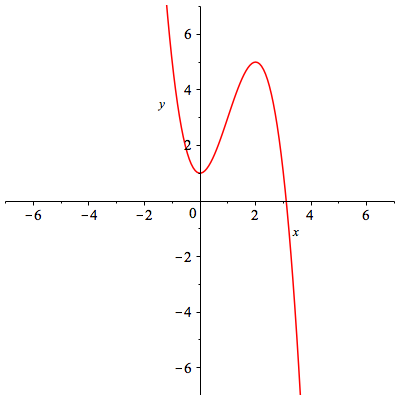
\includegraphics[width=0.7\textwidth]{images/-x^3+3x^2+1.png}
	\end{figure}
\end{myexample}
\newpage
\begin{myexample}
Von einer ganzrationalen Funktion 4. Grades wissen wir, dass ihr Graph im Ursprung eine horizontale Tangente besitzt und $W(1/-1)$ ein Wendepunkt ist, wobei die Wendetenagente durch den Punkt $P(0/1)$ läuft.\\
Bestimme mit Hilfe von Maple die Funktionsvorschrift, diskutiere dann die Funktion und suche die Wertemenge.
	\begin{equation*}f(x) = ax^4+bx^3+cx^2+dx+e\end{equation*}
	\begin{enumerate}
	\item  
    		\begin{align*}  
    			f(0) = 0
   		\end{align*}
	\item  
    		\begin{align*}  
    			f'(0) = 0
   		\end{align*}    
	\end{enumerate}
	oder
	\begin{eqnarray*}
		f(x) &=& x^2(ax^2+bx+c)
		\shortintertext{da}
		x &=& 0
	\end{eqnarray*}
	Eine doppelte Nulstelle ist
	\begin{enumerate}
	\item  
    		\begin{align*}  
    			f''(1) = 0
   		\end{align*}
	\item  
    		\begin{align*}  
    			f(1) = -1
   		\end{align*}    
   		% BILD TODO
   		BILD TODO
	\item
		\begin{align*}  
    			f'(1) = -2
   		\end{align*}    
	\end{enumerate}
	Mit Maple finden wir
	\begin{eqnarray*}
		f: \R \to \R \text{ text } f(x) = x^4-2x^2
		\shortintertext{\underline{Nullstellen:}}
		x_1 = 0, x_2 = 2
		\shortintertext{\underline{Extremalwerte:}}
		x_1 = 0, x_3 = \frac{3}{2}\\
		\to  f(x_3) = -\frac{27}{10}
		\shortintertext{\underline{Wendepunkt:}}
		x_1 = 0\\
		\to (0/0) \text{ ist ein Terassenpunkt}\\
		x_4 = 1\\
		\to f(x_4) = -1\\
		\shortintertext{\underline{Graph:}}
	\end{eqnarray*}
		\begin{figure}[H]
			\centering
			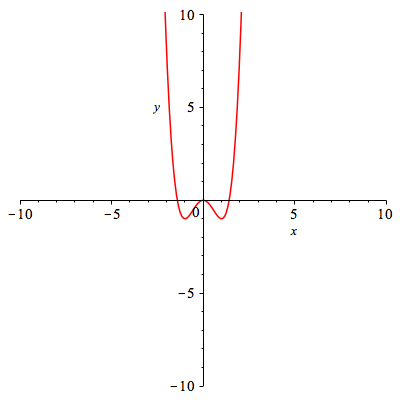
\includegraphics[width=0.7\textwidth]{images/x^4-2x^2.png}
		\end{figure}
		\begin{equation*}\text{Wertemenge: Wf}=[-\frac{27}{10}; \infty[\end{equation*}
\end{myexample}
\newpage
% 12.11.2014

\newpage
\section{Extremalwertprobleme}
Stellen wir uns die Frage nach dem kleinsten Benzinverbrauch, dem grössten Gewinn usw. und gelingt es uns, das Problem mit Hilfe einer Funktion zu formulieren, so können wir die Lösung mit der Differenzialrechnung finden.
\\\\TODO\\\\
Wie müssen wir Länge und Breite wählen, um mit 400m Maschendrahtzaun die grösstmögliche Fläche zu umzäunen?
\begin{enumerate}
\item \underline{Gesuchte Grösse berechnen}
\begin{equation*}F = a \cdot b\end{equation*}
\item \underline{Eine der auftretenden Grössen als Variable wählen}
\begin{quote}$b$ sei die Variable\end{quote}
\item \underline{Alle anderen Grössen mit Hilfe der Variablen und den bekannten Werten bestimmen}
\begin{eqnarray}a + 2b & = & 400 \nonumber \\
a & = & 400 - 2b\end{eqnarray}
\item \underline{Funktion und Definitionsmenge bestimmen}
\begin{eqnarray}F(b) & = & (400 - 2b) \cdot b\nonumber \\
& = & 400b - 2b^2\end{eqnarray}
mit
\begin{eqnarray}D_f & = & \{ b \quad | \quad 0 < b < 200 \quad \land \quad b \in \mathbb{R}\}\nonumber \\
& = & ]0;200[\end{eqnarray}
\\\\TODO: Graphs\\\\
\item \underline{Extremwerte berechnen}
\begin{equation*}F'(b) = 400- 4b\end{equation*}
$F'(b)$ ist $0$, wenn $b = 100$
\item \underline{Lösung diskutieren und alle gesuchten Grössen berechnen}
\\\\$b \in D_f$ und mit $F''(b) = -4$ wird $F''(100) < 0$, also ist bei $b = 100$ ein lokales Maximum.\\
Also ist $b=100, a=200$ und $F_{max} = 20000$
\end{enumerate}
Wählen wir einen Halbkreis, also ist
\begin{quote}$U = 400 = r \cdot \pi \rightarrow r = \frac{400}{\pi}$\end{quote}
und so
\begin{equation*}F(Halbkreis) = \frac{r^2 \pi}{2} = \frac{\pi}{2}(\frac{400}{\pi})^2 = \frac{400^2}{2 \pi} = 25464,79\end{equation*}
\begin{myproof}Beweis der Ableitung $f'(x)$: Wir beweisen mit vollständiger Induktion.
\begin{enumerate}
\item Behauptung ist für $n=1$ wahr, denn
\begin{equation*}\frac{dx}{dy} = \lim_{h \to 0}\frac{(x+h)^1 - x^1}{h} = \frac{h}{h} = 1\end{equation*}
und
\begin{equation*}1 \cdot x^{1-1} = 1 \cdot x^0 = 1\end{equation*}
\item Voraussetzung:
\begin{equation*}\frac{(x+h)^n - x^n}{h} = n \cdot x^{n-1}\end{equation*}
Behauptung:
\begin{eqnarray}&&\lim_{h \to 0}\frac{(x+h)^{(n+1)} - x^{(n+1)}}{h} = n \cdot x^{n-1} \nonumber \\
& = & \lim_{h \to 0}\frac{x^{n+1}h^0 + (n+1)x^nh^1 + ... + (n+1)x^1h^n + x^0h^{n+1}-x^{(n+1)}}{h} \nonumber \\
& = & \lim_{h \to 0} (n+1) \cdot x^n + ... + x^0h^n \nonumber \\
& = & (n+1)x^n\end{eqnarray}
und
\begin{equation*}(n+1) \cdot x^{(n+1)-1} = (n+1) x^n\end{equation*}
\item Nach (1) gilt die Behauptung für $n=1$ und nach (2) gilt sie für $n+1$, falls sie für $n$ gilt. Also gilt sie für $n = 2$ und nach (2) für $n+1$, ist 3 usw. Also gilt die Behauptung für alle $n \in \mathbb{N}$. \end{enumerate}
\qed\end{myproof}
\newpage
\begin{myexample}
	Ein rechteckiges Blech mit Länge $l= 8$ und Breite $b= 5$ soll zugeschnitten werden, dass daraus eine Schachtel ohne Deckel mit maximalen Volumen entsteht.\\
	\begin{figure}[H]
			\centering
			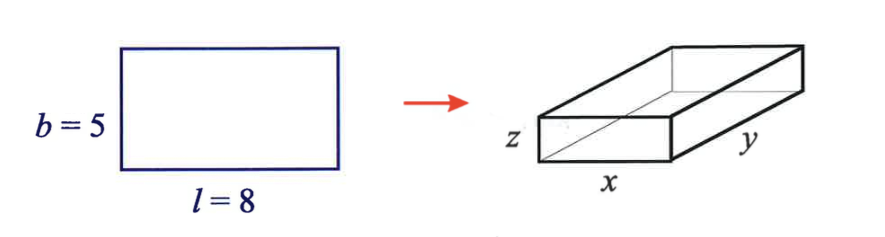
\includegraphics[width=\textwidth]{images/extremalwertproblem1.png}
	\end{figure}
	\begin{enumerate}
		\item
		\begin{equation*}V = xyz\end{equation*}
		\item
		z sei die Variable\\
		dann ist
		\begin{eqnarray*}
			x = 8-2z\\
			y = 5-2z
		\end{eqnarray*}
		und damit
		\item
		\begin{eqnarray*}
			V(z) &=& (8-2z)(5-2z)z\\
			&=& (40-16z-10+4z^2)z \\
			&=& 4z^3-26z2+40z\\
		\end{eqnarray*}
		\item
		mit
		\begin{equation*}D_v = ]0;2,5[\end{equation*}
		\item
		Also
		\begin{eqnarray*}
			V'(z) = 12z^2-52z+40
			\shortintertext{und}
			V'(z) = 0
			\shortintertext{wenn}
			3z^2-13z+10=0\\
			(3z-10)(z-1) = 0\\
			z_1 = \frac{10}{3}, z_2 = 1
		\end{eqnarray*}
		\item
		\begin{equation*}z_1 \not \in D_v \text{ aber } z_2 \in D_v\end{equation*}
		Mit
		\begin{eqnarray*}
			V''(z) = -24-52\\
			\shortintertext{wird}
			V''(1) < 0
			\shortintertext{also ist}
			z = 1
			\shortintertext{und damit}
			x = 6, y = 3\\
			v_{max} = 18
		\end{eqnarray*}
	\end{enumerate}
\end{myexample}
\newpage
\begin{myexample}
	Welche Höhe $h$ muss ein gerader Kegel haben, wenn er einer Kugel mit gegebenen Radius $R$ enbeschrieben ist und maximales Volumen besitzen soll?\\
	\begin{figure}[H]
			\centering
			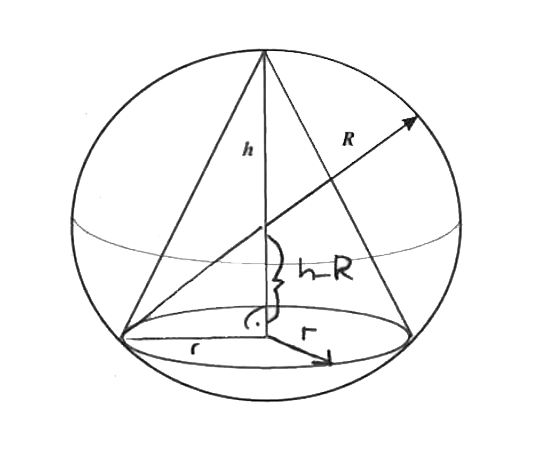
\includegraphics[width=0.7\textwidth]{images/extremalwertproblem2.png}
	\end{figure}
	\begin{enumerate}
		\item
		\begin{equation*}V = \frac{G\cdot h}{3}= \frac{r^2\cdot \Pi \cdot h}{3}\end{equation*}
		\item
		h sei die Variable, dann ist
		\begin{eqnarray*}
			R^2 &=& r^2 + (h-R)^2\\
			R^2 &=& r^2 + h^2 -2Rh+ R^2\\
			r^2 &=& 2RH-h^2
		\end{eqnarray*}
		und damit
		\item
		\begin{eqnarray*}
			V(h)&=& \frac{(2Rh-h^2)\cdot h\Pi}{3}\\
			&=& \frac{\Pi}{3}(2Rh^2-h^3)
		\end{eqnarray*}
		\item
		mit 
		\begin{equation*}D_v = ]0;2R[\end{equation*}
		
		wird
		\item
		\begin{eqnarray*}
			V'(h) &=& \frac{\Pi}{3}(4Rh-3h^2)
			\shortintertext{und}
			V'(h) &=& 0
			\shortintertext{wenn}
			h(4R-3h) &=& 0\\
			h_1 = 0 &\lor& 4R = 3h \to h_2 = \frac{4R}{3}
		\end{eqnarray*}
		\item
		\begin{equation*}h_1 \not \in D_v, \text{ aber } h_2 \in D_v\end{equation*}
		und mit
		\begin{eqnarray*}
			V''(h) &=& \frac{\Pi}{3}(4R-6h)
			\shortintertext{wird}
			V''(h_2) &=& \frac{\Pi}{3}(4R-6\cdot\frac{4R}{3})\\
			&=& \frac{\Pi}{3}(4R-8R) < 0
			\shortintertext{Also ist}
			h &=& \frac{4R}{3}
			\shortintertext{und damit}
			V_{max} &=& \frac{\Pi}{3}(2R\cdot \frac{16R^2}{9}-\frac{64R^3}{27})\\
			&=& \frac{3}{\Pi} \cdot \frac{96R^3-64R^3}{27}\\
			&=& \frac{32R^3\Pi}{81}
		\end{eqnarray*}
	\end{enumerate}
\end{myexample}
\newpage
\begin{myexample}
	Auf der Grundfläche eines geraden Drehkegels mit Kreisradius $R$ und Höhe $H$ steht ein Drehzylinder, welcher dem Kegel einbeschrieben ist.\\
	Welchen Radius muss dieser Zylinder haben, damit sein Volumen maximal wird?\\
	Wie gross wird dann dieses Volumen?\\
	\begin{figure}[H]
			\centering
			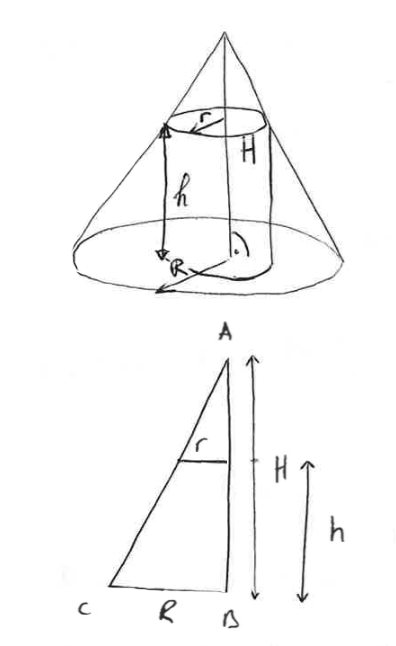
\includegraphics[width=0.4\textwidth]{images/extremalwertproblem3.png}
	\end{figure}
	\begin{enumerate}
		\item
			\begin{equation*}V = r^2\Pi h\end{equation*}
			und r sei die Variable.
		\item
			Mit der Ähnlichkeit des Dreiecks $ABC$ und $AB_1C$
			\begin{equation*}\frac{R}{r} = \frac{H}{H-h}\end{equation*} 
			und
		\begin{equation*}\frac{R^2\Pi}{r^2\Pi} = \frac{H^2}{(H-R)^2}\end{equation*}
			also
			\begin{eqnarray*}
				R(H-h) &=& rH\\
				RH-Rh &=& rH\\
				Rh &=& RH-rH\\
				h &=& \frac{H(R-r)}{R}
			\end{eqnarray*}
			und damit
		\item
			\begin{equation*}V(r) = \Pi r^2 \frac{H(R-r)}{R}\end{equation*}
			wird
		\item
			\begin{equation*}D_v = ]0;R[\end{equation*}
		\item
			\begin{eqnarray*}
				V(r) &=& \frac{\Pi}{R}(HRr^2-Hr^3)\\
				&=&\frac{H\Pi}{R}(Rr^2-r^3)
				\shortintertext{so wird}
				&=& V'(r) = \frac{H\Pi}{R}(R\cdot 2r-3r^2)
				\shortintertext{und}
				V'(h) = 0
				\shortintertext{wenn}
				r(2R-3r) = 0\\
				r_1 = 0 \text{ oder } r_2 = \frac{2R}{3}
			\end{eqnarray*}
		\item
			\begin{eqnarray*}
				r_1 \not \in D_v &aber& r_2 \in D_v
				\shortintertext{und damit}
				V''(r) &=& \frac{H\Pi}{R}(2R-6r)
				\shortintertext{wird}
				V''(r_2) &<& 0\\
				\shortintertext{also wird}
				r &=& \frac{2R}{3}
				\shortintertext{und}
				V_{max} &=& \frac{H\cdot T}{R}(R\cdot \frac{4R^2}{9}-\frac{8R^3}{27})\\
				&=& H \cdot \Pi (\frac{4R^2}{9} - \frac{8R^2}{27})\\
				&=&\frac{H\cdot\Pi\cdot4R^2}{27}
			\end{eqnarray*}
	\end{enumerate}
\end{myexample}
\newpage
% 19.11.2014
\section{Winkelfunktionen, Produktregeln, Kettenregel}
\subsection{Winkelfunktionen}
Die Winkelfunktionen sind \underline{periodisch}, und zwar
\begin{eqnarray*}
	\sin(x+k\cdot2\Pi) &=& \sin(x)\\
	\cos(x+k\cdot2\Pi) &=& \cos(x)\\
	\tan(x + k\cdot \Pi) &=& \tan(x)\\
	k &\in& \Z
\end{eqnarray*}
Ist 
\begin{equation*}f: \R \to [-1;1] \text{mit} t(x) = \sin(x)\end{equation*}
so ist
\begin{equation*}f'(x) = \lim_{h \to 0}\frac{\sin(x+h) - \sin x}{h}\end{equation*}
und
\begin{equation*}\sin \alpha - \sin \beta = 2 \cdot \cos(\frac{\alpha + \beta}{2}) \cdot \sin(\frac{\alpha - \beta}{2})\end{equation*}
wird
\begin{eqnarray}\sin(x+h) - \sin x & = & 2 \cdot \cos(\frac{x+h+x}{2}) \cdot \sin(\frac{(x+h)-x}{2}) \nonumber \\
& = & 2 \cdot \cos(\frac{2x + h}{2}) \sin(\frac{h}{2})\end{eqnarray}
und damit
\begin{eqnarray}f'(x) & = & \lim_{h \to 0} \frac{1}{h} \cdot (2\cos(\frac{2x+h}{2}) \cdot \sin(\frac{h}{2}) \nonumber \\
& = & \lim_{h \to 0} \frac{2}{h} \cdot (\cos(\frac{2x+h}{2}) \cdot \sin(\frac{h}{2}) \nonumber \\
& = & \lim_{h \to 0} \cos(\frac{2x + h}{h}) \cdot \frac{\sin(\frac{h}{2})}{\frac{h}{2}}\end{eqnarray}
Um $\lim_{h \to 0} \frac{\sin \frac{h}{2}}{\frac{h}{2}}$ zu bestimmen, betrachten wir den Sinus im Einheitskreis bei $0$.
\\\\TODO: Zeichnung\\\\
Ist $\alpha$ im Bogenmass, so ist
\begin{equation*}\sin \alpha < \alpha < \tan \alpha\end{equation*}
\begin{equation*}\sin \alpha < \alpha < \frac{\sin \alpha}{\cos \alpha}\end{equation*}
\begin{equation*}1 < \frac{\alpha}{\sin \alpha} < \frac{1}{\cos \alpha}\end{equation*}
\begin{equation*}1 > \frac{\sin \alpha}{\alpha} > \cos \alpha\end{equation*}
\begin{equation*}1 \geq \lim_{\alpha \to 0} \frac{\sin \alpha}{\alpha} \geq \lim_{\alpha \to 0} \cos \alpha\end{equation*}
\begin{equation*}1 \geq \lim_{\alpha \to 0} \frac{\sin \alpha}{\alpha} \geq 1\end{equation*}
\begin{equation*}\boxed{\lim_{\alpha \to 0} \frac{\sin \alpha}{\alpha} = 1}\end{equation*}
Schliesslich finden wir
\begin{eqnarray}f'(x) & = & \lim_{h \to 0} \cos \frac{2x+h}{2} \cdot \frac{\sin \frac{h}{2}}{\frac{h}{2}} \nonumber \\
& = & \cos x \cdot 1 \nonumber \\
& = & \cos x\end{eqnarray}
\begin{equation*}\boxed{f(x) = \sin x \quad \to \quad f'(x) = \cos x}\end{equation*}
Analog finden wir
\begin{equation*}\boxed{g(x) = \cos x \quad \to \quad g'(x) = -\sin x}\end{equation*}
\begin{myexample}\begin{enumerate}
\item 
	\begin{eqnarray}f(x) & = & x^2 + 3 \cdot \cos x \nonumber \\
	\to f'(x) & = & 2x - 3 \cdot \sin x\end{eqnarray}
\item 
	\begin{eqnarray}\lim_{\alpha \to 0} \frac{\sin (7 \alpha)}{4 \alpha} & = & \lim_{\alpha \to 0} 		\frac{\frac{7}{4} \sin(7 \alpha)}{\frac{7}{4} \cdot 4 \alpha} \nonumber \\
& = & \lim_{\alpha \to 0} \frac{\frac{7}{4} \sin(7 \alpha)}{7 \alpha} \nonumber \\
& = & \frac{7}{4} \lim_{\alpha \to 0} \frac{\sin(7\alpha)}{7 \alpha} \nonumber \\
& = & \frac{7}{4} \cdot 1 = \frac{7}{4}\end{eqnarray}
\item \begin{eqnarray}\lim_{\beta \to 0} \frac{\sin(2\beta)}{cos \beta} & = & \lim_{\beta \to 0} \frac{2 \sin \beta \cos \beta}{\cos \beta} \nonumber \\
& = & \lim_{\beta \to 0} 2 \sin \beta = 0\end{eqnarray}
\item
	Suche die Extremwerte von
	\begin{eqnarray*}
		f: \R \to \R \text{ mit } f(x) &=& \cos(x)-x\\
		f'(x) &=& -\sin(x) -1
		\shortintertext{und}
		f'(x) &=& 0
		\shortintertext{wenn}
		\sin(x) &=& -1\\
		x &=& \frac{3\Pi}{2}\\
		x &=& \frac{3\Pi}{2} + k\cdot 2\Pi, k \in \Z
		\shortintertext{so wird}
		f(x_1) &=& f(\frac{3\Pi}{2}) \\
		&=& \cos\frac{3\Pi}{2}-\frac{3\Pi}{2}\\
		&=& -\frac{3\Pi}{2}\\
		f(x_2) &=& f(\frac{3\Pi}{2}+2\Pi)\\
		&=& \cos(\frac{3\Pi}{2}+2\Pi) -(\frac{3\Pi}{2}+2\Pi)\\
		&=& -\frac{3\Pi}{2}-2\Pi
	\end{eqnarray*}
\end{enumerate}
\end{myexample}
\newpage
\subsection{Produktregeln}
Die Funktion
\begin{equation*}h: \R \to \R  \text{ mit } h(x) = x^2 \cdot \sin(x)\end{equation*}
ist das Produkt der Funktionen
\begin{equation*}f(x) = x^2 \text{ und } g(x) = \sin(x)\end{equation*}
Wir finden die Ableitung eines Produktes mit
\begin{eqnarray*}h'(x) & = & \lim_{h \to 0} \frac{f(x+h) \cdot g(x+h) - f(x)g(x)}{h} \nonumber \\
& = & \lim_{h \to 0} \frac{f(x+h) \cdot g(x+h) - f(x) \cdot g(x+h) + f(x)\cdot g(x+h) - f(x)g(x)}{h} \nonumber \\
& = & \lim_{h \to 0} \frac{f(x+h)g(x+h) - f(x)g(x+h)}{h} + \frac{f(x)g(x+h)-f(x)g(x)}{h} \nonumber \\
& = & \lim_{h \to 0} \frac{f(x+h)-f(x)}{h} g(x+h)+f(x) \cdot \frac{g(x+h)-g(x)}{h} \nonumber \\
& = & f'(x) \cdot g(x) + f(x) \cdot g'(x)
\end{eqnarray*}
Damit finden wir die Produktregel:
{\begin{equation*}\boxed{(fg)' = f'g + fg'}\end{equation*}}
\begin{myexample}Berechne die Ableitung von
\begin{enumerate}
\item
\begin{eqnarray*}
	h(x) &=& x^2 \cdot \sin(x)
	\shortintertext{Mit}
	f(x) &=& x^2\\
	g(x) &=& \sin(x)
	\shortintertext{wird}
	f'(x) &=& 2x\\
	g'(x) &=& \cos(x)
	\shortintertext{und damit}
	h'(x) &=& x^2\cos(x) + 2x\sin(x)
\end{eqnarray*}
\item 
\begin{eqnarray*}
	f(x) & = & x^2 \cdot \cos(x) \\
	u(x) & = & x^2 \\
	v(x) & = & \cos(x)
\end{eqnarray*}
Mit
\begin{eqnarray*}
	u'(x) & = & 2x \nonumber \\
	v'(x) & = & -\sin(x)
\end{eqnarray*}
finden wir
\begin{eqnarray*}
	f'(x) & = & 2x \cdot \cos(x) + x^2 \cdot (-\sin(x)) \nonumber \\
	& = & 2x \cdot \cos(x) - x^2 \cdot \sin(x)
\end{eqnarray*}
\item
\begin{eqnarray*}
	g(x) & = & \sin(2x) \\
	&=&  2 \sin(x) \cos(x) \nonumber \\
	g'(x) &= & 2(\cos^2(x) - \sin^2(x)) \nonumber \\
	& = & 2 \cos(2x)
\end{eqnarray*}
\end{enumerate}
\end{myexample}
\newpage
\subsection{Kettenregel}
Betrachten wir die folgende Funktion
\begin{eqnarray*}
	k(x) &=& \sin(3x)\\
	\shortintertext{Mit}
	k(x) &=& 3\sin(x)-4\sin^3(x)\\
	\shortintertext{müssen wir zuerst}
	l(x) &=& \sin^3x
	\shortintertext{ableiten}
	l(x) &=& \sin x \cdot \sin^2x\\
	l'(x)&=& \sin x (\sin^2x)' + \cos x\cdot\sin^2x\\
	&=& \sin x(\sin x \cdot \cos x + \cos x \cdot \sin x) + \cos x \cdot \sin^2x\\
	&=& 2\sin^2 x\cos x + \cos x \sin^2 x\\
	&=& 3 \sin^2(x)\cos(x)
	\shortintertext{und so}
	k'(x) &=& 3 \cos x -4\cdot 3 \sin^2x\cos x\\
	&=& 3 \cos x(1-4\sin^2x)\\
	&=& 3 \cos x(1-4(1-\cos^2x))\\
	&=& 3 \cos x(1-4 + 4 \cos^2x)\\
	&=& 3 \cos x(4 \cos^2x-3)\\
	&=& 3(4\cos^3x-3\cos x)\\
	&=& 3 \cos 3x
\end{eqnarray*}
Zusammenfassung
\begin{eqnarray*}
	f(x) &=& \sin(2x) \to f'(x) = 2 \cos 2x\\
	g(x) &=& \sin(3x) \to g'(x) = 3 \cos 3x\\
	h(x) &=& \sin(4x) \to h'(x) = 4 \cos 4x\\
	\ldots&&	
	\shortintertext{also}
	(\sin kx)' &=& k\cos(kx), k \in \Q
	\shortintertext{analog}
	(\cos kx)' &=& -k\sin(kx), k \in \Q
\end{eqnarray*}
\newpage
\noindent
Weiter haben wir gefunden
\begin{eqnarray*}
	f(x) &=& \sin^2x \to f'(x) = 2\sin x\cos x\\
	g(x) &=& \sin^3x \to g'(x) = 3\sin^2x \cdot \cos x
	\shortintertext{also}
	(\sin^nx)' &=& n\sin^{n-1}x\cdot \cos(x), n \in \N
	\shortintertext{und}
	f(x) &=& \cos^2x \to f'(x) = -2\cos x \sin x\\
	g(x) &=& cos^3x \to g'(x) = -3\cos^2x\sin x
\end{eqnarray*}
Was wir hier gefunden haben, ist die Anwendung der \textbf{Kettenregel}.\\
\\
Ist
\begin{eqnarray*}
	h(x) &=& g(f(x))
	\shortintertext{so ist}
	h'(x) &=& g'(u)\cdot f'(x) \text{ mit } u = f(x)
\end{eqnarray*}
Wir nennen $f'(x)$ die \underline{innere Abletung}.
\begin{myexample}
	\begin{enumerate}
		\item
			\begin{eqnarray*}
				h(x) &=& \sin^4x
				\shortintertext{So ist}
				f(x) &=& \sin x, g(u) = u^4\\
				h'(x) &=& 4u^3 \cos x
				\shortintertext{also}
				h'(x) &=& 4\sin^3x \cos x
			\end{eqnarray*}
		\item
			\begin{eqnarray*}
				i(x) &=& (x^3 + 2x^2 -4)^8\\
				i'(x) &=& 8(x^3 + 2x^2 -4)^7\cdot(3x^2+4x)
			\end{eqnarray*}		
	\end{enumerate}
\end{myexample}
% 9.12.2014%
\chapter{Integralrechnung}
\section{Stammfunktion}
Wir kennen die Abbildung $f'$ einer Funktion $f$ und suchen die Funktion $f(x)$.\\
\begin{myexample}
	\begin{enumerate}
		\item
		\begin{eqnarray*}
			f'(x) &=& \cos x\\
			\to f(x) &=& \sin x
		\end{eqnarray*}
		\item
		\begin{eqnarray*}
			g'(x) &=& x^3 \\
			\to g(x) &=& \frac{x^4}{4}\\
			\shortintertext{oder}
			&&\frac{x^4}{4} + 5\\
			\shortintertext{oder}
			&&\frac{x^4}{4} -7\\
			\shortintertext{etc.}
		\end{eqnarray*}
	\end{enumerate}
\end{myexample}
\noindent
Ist $f(x)$ die Ableitung einer Funktion $F(x)$, so heisst $F$ eine \underline{Stammfunktion} von $f$:
\begin{equation*}F'(x) = f(x)\end{equation*}
\begin{myexample}
	\begin{eqnarray*}
		f(x) &= &x^2+4x+1\\
		\to F(x) &=& \frac{x^3}{3} + 2 x^2+ C, C \in \R
	\end{eqnarray*}
\end{myexample}
\noindent
Zu einer Funktion f gibt es also beliebig viele Stammfunktionn. Sie unterscheiden sich duch eine Konstante C.\\
\begin{mydef}
	Die Menge aller Stammfunktionen heisst \underline{unbestimmtes Integral}, wofür wir
	\begin{equation*}\int \! f(x) \, \mathrm{d} x = F(x) + C\end{equation*}
	schreiben. Dabei heisst
	\begin{itemize}
		\item $f(x)$ der \underline{Integrand}
		\item $\mathrm{d}x$ das \underline{Differential}
		\item $C \in \mathbb{R}$ die \underline{Integrationskonstante}
	\end{itemize}
\end{mydef}
\begin{myexample}
\begin{enumerate}
Wir berechnen die unbestimmten Integrale:
\item\begin{equation*}\int \! x^2dx = \frac{x^3}{3}+C\end{equation*}
\item \begin{equation*}\int \! 4x^3 - 3x \, \mathrm{d} x = x^4 - \frac{3x^2}{2} + C\end{equation*}
\item \begin{equation*}\int \! 2 \cos(x) + 3 \sin(x) \, \mathrm{d} x = 2 \sin(x) - 3\cos(x) + C\end{equation*}
\item \begin{equation*}\int \! at^2 + bt + c \, \mathrm{d} t = a \frac{t^3}{3} + b \frac{t^2}{2} + ct + D\end{equation*}
\begin{equation*}\int \! at^2 + bt + c \, \mathrm{d} a = \frac{a^2}{2} \cdot \frac{t^2}{2} + bta + ca + D\end{equation*}
\end{enumerate}
\end{myexample}
\newpage
\noindent
Mit Hilfe der Differenzialrechnung finden wir die regeln für die Integralrechnung.\\
\\
Regeln:
\begin{enumerate}
\item \begin{equation*}\int \! f(x) + g(x) \, \mathrm{d} x = \int \! f(x) \, \mathrm{d} x + \int \! g(x) \, \mathrm{d} x\end{equation*}
\item \begin{equation*}k \in \mathbb{R}: \int \! k \cdot f(x) \, \mathrm{d} x = k \cdot \int \! f(x) \, \mathrm{d} x\end{equation*}
\item 
\begin{eqnarray*}
	\int \! x^p \, \mathrm{d} x = \frac{x^{p+1}}{p+1} + C\quad ; \quad p \in \mathbb{R} \setminus \{-1\}
	\shortintertext{Anmerkung}
	\int  x^{-1}dx = \int \frac{1}{x}dx = \int \frac{dx}{x} = ln|x|+ C
\end{eqnarray*}
\end{enumerate}
\begin{myexample}
	\begin{enumerate}
		\item
			\begin{eqnarray*}
				&&\int \frac{2}{x^2}+3x^4dx\\
				&=& \int 2x^{-2}dx +  3x^4dx\\
				&=&  2\int x^{-2}dx+3\int x^4dx\\
				&=& 2\frac{x^{-1}}{-1}+3\frac{x^5}{5}+C\\
				&=& \frac{-2}{x} + \frac{3x^5}{5}+C 
			\end{eqnarray*}
		\item
			\begin{eqnarray*}
				&& \int \sqrt{x} +x+1dx\\
				&=& \int x^{\frac{1}{2}} + x + 1dx\\
				&=& \frac{2x^{\frac{3}{2}}}{3}+\frac{x^2}{2}+x+C\\
				&=& \frac{2}{3}\sqrt{x^3}+\frac{x^2}{2}+x+C\\
			\end{eqnarray*}
		\item
			\begin{eqnarray*}
				&&\int a^2b^2+ab^3db\\
				&=& a^2\frac{b^3}{3}+a\frac{b^4}{4}+C
			\end{eqnarray*}
		\item
		Mithilfe der Ableitungen der Winkelfunktionen finden wir
			\begin{eqnarray*}
				&& \int \sin(kx)dx\\
				&=& -\frac{\cos(kx)}{k}+C
				\shortintertext{und}
				&&\int\cos(kx)dx\\
				&=& \frac{\sin(kx)}{k} + C; k\in R \backslash \{0\}
			\end{eqnarray*}
	\end{enumerate}
\end{myexample}
\newpage
\section{Flächeninhalte}
Welchen Inhalt besitzt die durch den Graphen von
\begin{equation*}f: \mathbb{R} \to \mathbb{R}_0^+ \quad \mbox{mit} \quad f(x) = x^2\end{equation*}
die Gerade $x=b$ $(b > 0)$ und die x-Achse begrenzte Fläche?
\\\\TODO: Grafik\\\\
Wir wählen n Rechtecke mit Breite $\frac{b}{n}$, und zwar solche die ''zu gross'' sind mit Flächeninhalt $F_1,F_2,F_3,F4_, \ldots, F_n$ und solche die ''zu klein'' sind mit Flächeninhalt $f_1,f_2,f_3,f_4,\ldots,f_n$
Es ist
\begin{eqnarray*}
	F_1 &=& \frac{b}{n} \cdot f(\frac{b}{n}) = \frac{b}{n} (\frac{b}{n})^2 = \frac{b^3}{n^3}\\
	F_2 &=& \frac{b}{n} \cdot f(\frac{2b}{n}) = \frac{b}{n} \cdot (\frac{2b}{n})^2 = 2^2 \cdot \frac{b^3}{n^3}\\
	F_3 &=& \frac{b}{n} \cdot f(\frac{3b}{n}) = \frac{b}{n} \cdot (\frac{3b}{n})^2 = 3^2 \cdot \frac{b^3}{n^3}\\
	\ldots&&\\
	F_n &=& \frac{b}{n} \cdot f(\frac{n \cdot b}{n}) = \frac{b}{n} \cdot b^2 = n^2 \cdot \frac{b^3}{n^3}
\end{eqnarray*}
und damit ist die erste Näherung die \underline{Obersumme}.\\
\begin{eqnarray} 
	O_n &=& F_1 + F_2 + ... + F_n \notag\\
	&=& \frac{b^3}{n^3} + 2^2 \cdot \frac{b^3}{n^3} + 3^2 \cdot \frac{b^3}{n^3} + ... + n^2\cdot\frac{b^3}{n^3} \notag\\
	&=& \frac{b^3}{n^3}(1+2^2+3^3+\ldots+n^2) \label{eq:Obermenge}
\end{eqnarray}
Weiter ist
\begin{eqnarray*}
	f_1 = 0, f_2 = F_1, f_3 = F_2, \ldots, f_n = F_n-1
	\shortintertext{also}
	f_2 = \frac{b^3}{n^3}, f_3 = \frac{b^3}{n^3} \cdot 2^2, \ldots, f_n = \frac{b^3}{n^3} (n-1)^2
\end{eqnarray*}
und damit wird die \underline{Untersumme} der ersten Näherung
\begin{eqnarray} 
	U_n &=& f_1+f_2+f_3+\ldots+f_n \notag\\
	&=& 0 +\frac{b^3}{n^3}+ \frac{b^3}{n^3} \cdot 2^2+ \ldots + \frac{b^3}{n^3} (n-1)^2 \notag\\
	&=& \frac{b^3}{n^3}(1+2^2+3^2+\ldots+(n-1)^2) \label{eq:Untermenge}
\end{eqnarray}
Setzen wir 
\begin{equation*}1^2+2^2+3^2+\ldots+n^2= \frac{n(2n+1)(n+1)}{6}\end{equation*}
in ~\ref{eq:Obermenge} ein, so erhalten wir
\begin{eqnarray}
	O_n &=& \frac{b^3}{n^3} \cdot \frac{n(2n+1)(n+1)}{6} \notag\\
	&=& \frac{b^3}{n^2} \cdot \frac{(2n+1)(n+1)}{6}\notag\\
	&=&\frac{b^3}{6} \cdot \frac{(2n+1)(n+1)}{n^2}\notag\\
	&=& \frac{b^3}{6}\cdot\frac{(2n+1)}{n}\cdot\frac{n+1}{n}\notag\\
	&=& \frac{b^3}{6}\cdot (2+\frac{1}{n})\cdot(1+\frac{1}{n}) \label{eq:Obermenge2}
\end{eqnarray}
Setzen wir
\begin{eqnarray*}
	1^2+2^2+3^2\ldots+(n-1)^2 &=& \frac{(n-1)(2(n-1)+1)(n-1+1)}{6}\\
	&=& \frac{(n-1)(2-1)(n)}{6}
\end{eqnarray*}
in  ~\ref{eq:Untermenge} ein, so erhalten wir
\begin{eqnarray}
	Un &=& \frac{b^3}{n^3}\cdot\frac{n(2n-1)(n-1)}{6} \notag\\
	&=& \frac{b^3}{6}\cdot \frac{n(2n-1)(n-1)}{n^2} \notag\\
	&=& \frac{b^3}{6}(2-\frac{1}{n})(1-\frac{1}{n}) \label{eq:Untermenge2}
\end{eqnarray}
lassen wir n wachsen, so erhalten wir eine nächste Näherung.\\
Wir bilden eine \underline{Intervallschachtelung} für den gesamten Flächeinhalt F:\\
\\
TO DO: BILD\\
\\
Dazu muss
\begin{enumerate}
	\item
		\begin{equation*}\forall n \> U_n+1 > U_n\end{equation*}
	\item
		\begin{equation*}\forall n\> O_{n+1} > O_n\end{equation*}
	\item
		\begin{equation*}\lim_{n\to \infty}(0-U_n) =0\end{equation*}
	\item
		\begin{equation*}\lim_{n\to \infty} U_n = \lim_{n\to\infty}O_n\end{equation*}
\end{enumerate}
erfüllt sein.\\
\\
Wir müssen nur noch 4. überprüfen.\\
Mit ~\ref{eq:Obermenge2} wird
\begin{eqnarray*}
	\lim_{n\to\infty}O_n &=& \lim_{n\to\infty} \frac{b^3}{6} (2+\frac{1}{n})(1+\frac{1}{n})\\
	&=& \frac{b^3}{6}\cdot 2\\
	&=& \frac{b^3}{3}
\end{eqnarray*} 
und mit ~\ref{eq:Untermenge2} 
\begin{eqnarray*}
	\lim_{n\to\infty}U_n &=& \lim_{n\to\infty} \frac{b^3}{6} (2-\frac{1}{n})(1-\frac{1}{n})\\
	&=& \frac{b^3}{6}\cdot 2\\
	&=& \frac{b^3}{3}
\end{eqnarray*} 
Alsi ist 
\begin{equation*}\underline{\underline{F = \frac{b^3}{3}}}\end{equation*}
 Es ist
 \begin{eqnarray*}
 	\int x^2dx &=& \frac{x^3}{3}+C
 	\shortintertext{und}
 	F &=& \frac{b^3}{3}
 \end{eqnarray*}
 deshalb schreiben wir
 \begin{equation*}\boxed{\int_0^b x^2dx= \frac{b^3}{3}}\quad \quad \mbox{"Integral von 0 bis b"}\end{equation*}
 welches wir ein \underline{bestimmtes Integral} mit der \\
 \begin{center}
 	unteren Grenze 0\\
 	oberen Grenze b\\
 \end{center}
nennen. Wir sagen auch Riemann-Integral.
\newpage
\section{Hauptsatz der Differential- und Integralrechnung}
Es ist
\begin{eqnarray*}
	\int_2^7x^2dx &=& \frac{7^3}{3}-\frac{2^3}{3}\\
	\shortintertext{Ist dann auch}
	\int_1^3x^3dx &=& \frac{3^4}{4}-\frac{1^4}{4}?\\
	\int_0^n\cos x dx &=& \sin \Pi - \sin 0
\end{eqnarray*}
\underline{Hauptsatz:} Ist f in $[a;b]$ integrierbar, so ist
\begin{eqnarray*}
	\int_a^bf(x)dx &=& F(b) -F(a)
	\shortintertext{wobei}
	F'(x) &=& f(x)
\end{eqnarray*}
\underline{Beweisidee:}\\
TO DO: BILD\\
\\
Ist $x_0$ variabel, so ist
\begin{eqnarray*}
	F(x_0) &=& \int^{x_0}_a f(x)dx
	\shortintertext{Dann ist}
	F(x_0+h)-F(x_0) &=& \int^{x_0+h}_{x_0} f(x)dx
	\shortintertext{Es gibt ein Rechteck mit Breite h und Länge $f(\xi)$, $x_0 < \xi < x_0 + h$, so dass}
	F(x_0+h)-F(x_0)&=& h \cdot f(\xi)\\
	\frac{F(x_0+h)-F(x_0)}{h} &=& f(\xi)\\
	\lim_{h\to 0} \frac{F(x_0+h)-F(x_0)}{h}  &=& \lim_{h\to 0} f(\xi)\\
	F'(x_0) &=& f(x_0)	
\end{eqnarray*}	
\underline{Regeln}
\begin{enumerate}
	\item
	\begin{equation*}\int_a^b f(x)dx + \int_b^c f(x)dx = ????\end{equation*}
	\item
	\begin{equation*}\int_a^b f(x)dx+ \int_a^b g(x)dx = \int_a^b f(x) + g(x) dx\end{equation*}
	\item
	\begin{equation*}\int_b^a f(x)dx = -\int_a^b f(x)dx\end{equation*}
	\item
	\begin{equation*}\int_a^a f(x)dx = 0\end{equation*}
\end{enumerate}
Wollen wir
\begin{equation*}\int_1^4 x^2+2x-3dx\end{equation*}
berechnen, so suchen wir eine Stammfunktion.\\
Um uns die Arbeit zu erleichtern wählen wir $C=0$.
\begin{equation*}
	F(x) = \frac{x^3}{3}+x^2-3x
\end{equation*}
Setzen 4 und 1 ein und subtrahieren.\\
Dafür schreiben wir
\begin{eqnarray*}
	\int_1^4 x^2+2x-3dx &=& \frac{x^3}{3}+x^2-3x \Big|_1^4\\
	&=& \frac{4^3}{3}+4^2-4\cdot 3 -(\frac{1^3}{3}+1^2-3\cdot 1)\\
	&=& \frac{64}{3} + 16 -12 - \frac{1}{3} -1 + 3\\
	&=& \underline{27}
\end{eqnarray*}
Es ist also
\begin{eqnarray*}
	\int_0^\Pi \sin(x)dx &=& -\cos(x) \Big|_0^\Pi\\
	&=& -\cos\Pi-(-\cos0)\\
	&=& 1 + 1\\	
	&=& 2
\end{eqnarray*}
TO DO: BILD
und 
\begin{eqnarray*}
	\int_0^{2\Pi} \sin(x)dx &=& -\cos(x) \Big|_0^{2\Pi}\\
	&=& -\cos2\Pi-(-\cos0)\\
	&=& -1 + 1\\	
	&=& 0
\end{eqnarray*}
TO DO: BILD
\begin{center}
	Das Integral ist 0\\
	Die Fläche ist 4.
\end{center}
Das bestimmte Integral ist negativ, wenn $f(x)$ negativ ist.
\begin{equation*}\int_{-1}^1 x^3dx = 0\end{equation*}
TO DO: BILD
\begin{myexample}
	\begin{eqnarray*}
		\int_0^{16} x-4\sqrt{x}dx &=& \frac{x^2}{2}-4\frac{x^{\frac{3}{2}}}{\frac{3}{2}}\Big|_0^{16}\\
		&=& \frac{x^2}{2} - \frac{8}{3}x \sqrt{x} \Big|_0^{16}\\
		&=& 128 - \frac{8}{3} \cdot 16 \sqrt{16}\\
		&=& 128 - \frac{512}{3} = \frac{384-512}{3} = - \frac{128}{3}
	\end{eqnarray*}
\end{myexample}
\newpage
\section{Zwei Graphen}
Suchen wir den Inhalt der Fläche , die durch 2 Graphen zwischen zwei aufeinanderfolgenden Schnittpunkte $x_1,x_2$ begrenzt ist,\\ \\
So ist
\begin{equation*}
	F = \int_{x_1}^{x_2}f(x)dx -\int_{x_1}^{x_2}g(x)dx = \int_{x_1}^{x_2}f(x)-g(x)dx
\end{equation*}
Ist
\begin{equation*}g(x) < 0 \text{ für } x \in[x_1;x_2]\end{equation*}
So wählen wir eine $\overline{x}$ Achse, so dass 
\begin{eqnarray*}
	g(\overline{x}) > 0  \text{ für } \overline{x} \in [x_1;x_2]
	\shortintertext{Dann ist}
	f(\overline{x}) = f(x) + k \\ 
	g(\overline{x}) = g(x) + k
	\shortintertext{und}
	F_2 = \int_{x_1}^{x_2} f(\overline{x}) -g(\overline{x}) d\overline{x}
	\shortintertext{also}
	F  = \int_{x_1}^{x_2}f(x)+k-(g(x)+k)dx\\
	\boxed{F =  \int_{x_1}^{x_2}f(x)-g(x)dx}
\end{eqnarray*}
\chapter{Kurzreferenz}
\section{Maximum, Minimum Graphen}
BILD TODO
 \section{Begriffe}
 \begin{tabularx}{\textwidth}{lX}
Schnittwinkel zweier Graphen & Unter dem Schnittwinkel zweier Graphen verstehen wir den Winkel zwischen den Tangen- ten im Schnittpunkt
\end{tabularx}
\end{document}